\chapter{基准工况流场分析}\label{chap:baseline}

\section{基准工况参数总结}\label{sec:baseline-params}

基线工况以He等\cite{he2024}文献报告最优工况为基础几何锚点进行建构，分别具有适中程度的喷嘴高度、喷嘴收缩角度、整形板长度以及整形板倾斜角度，具体数值总结在\cref{tab:3.1}中。其余工况在基线工况的基础上以可行域为宽度线性分布，每一组研究线包含4-5个工况，改变其中一个决定性变量进行模型重构。

\begin{table}[!htb]
  \centering
  \caption{基准工况几何参数与计算层高}\label{tab:3.1}
  \renewcommand{\arraystretch}{1.3}
  \begin{tabular}{ccccc}
    \toprule
    $\theta$ & $L$ & $TL$ & $\alpha$ & $H$ \\
    \midrule
    30° & 20 mm & 50 mm & 10° & 13.32 mm \\
    \bottomrule
  \end{tabular}
\end{table}

\section{速度场分析}

\subsection{喷嘴内速度分布与插塞流特征}

\cref{fig:3.1}展示了基准工况下喷嘴纵截面（XY平面）的速度分布云图以及入口直管段细节图。由图可见，浆体在入口直管段呈现出典型的黏塑性插塞流特征：中心区域流速均匀，截面速度梯度接近于零，对应局部剪切速率$\dot{\gamma} < \dot{\gamma}_c = 0.01~\text{s}^{-1}$，材料处于未屈服状态，形成宏观意义上的``刚性塞''；而近壁区域受固壁无滑移条件约束，速度迅速降低至零，该区域剪切速率显著高于截断值，浆体已发生屈服并产生流动。这种中心刚性、近壁流动的速度剖面是黏塑性流体在管道流动中的典型特征，与H-B流体理论预测一致。

\begin{figure}[!htb]
  \centering
  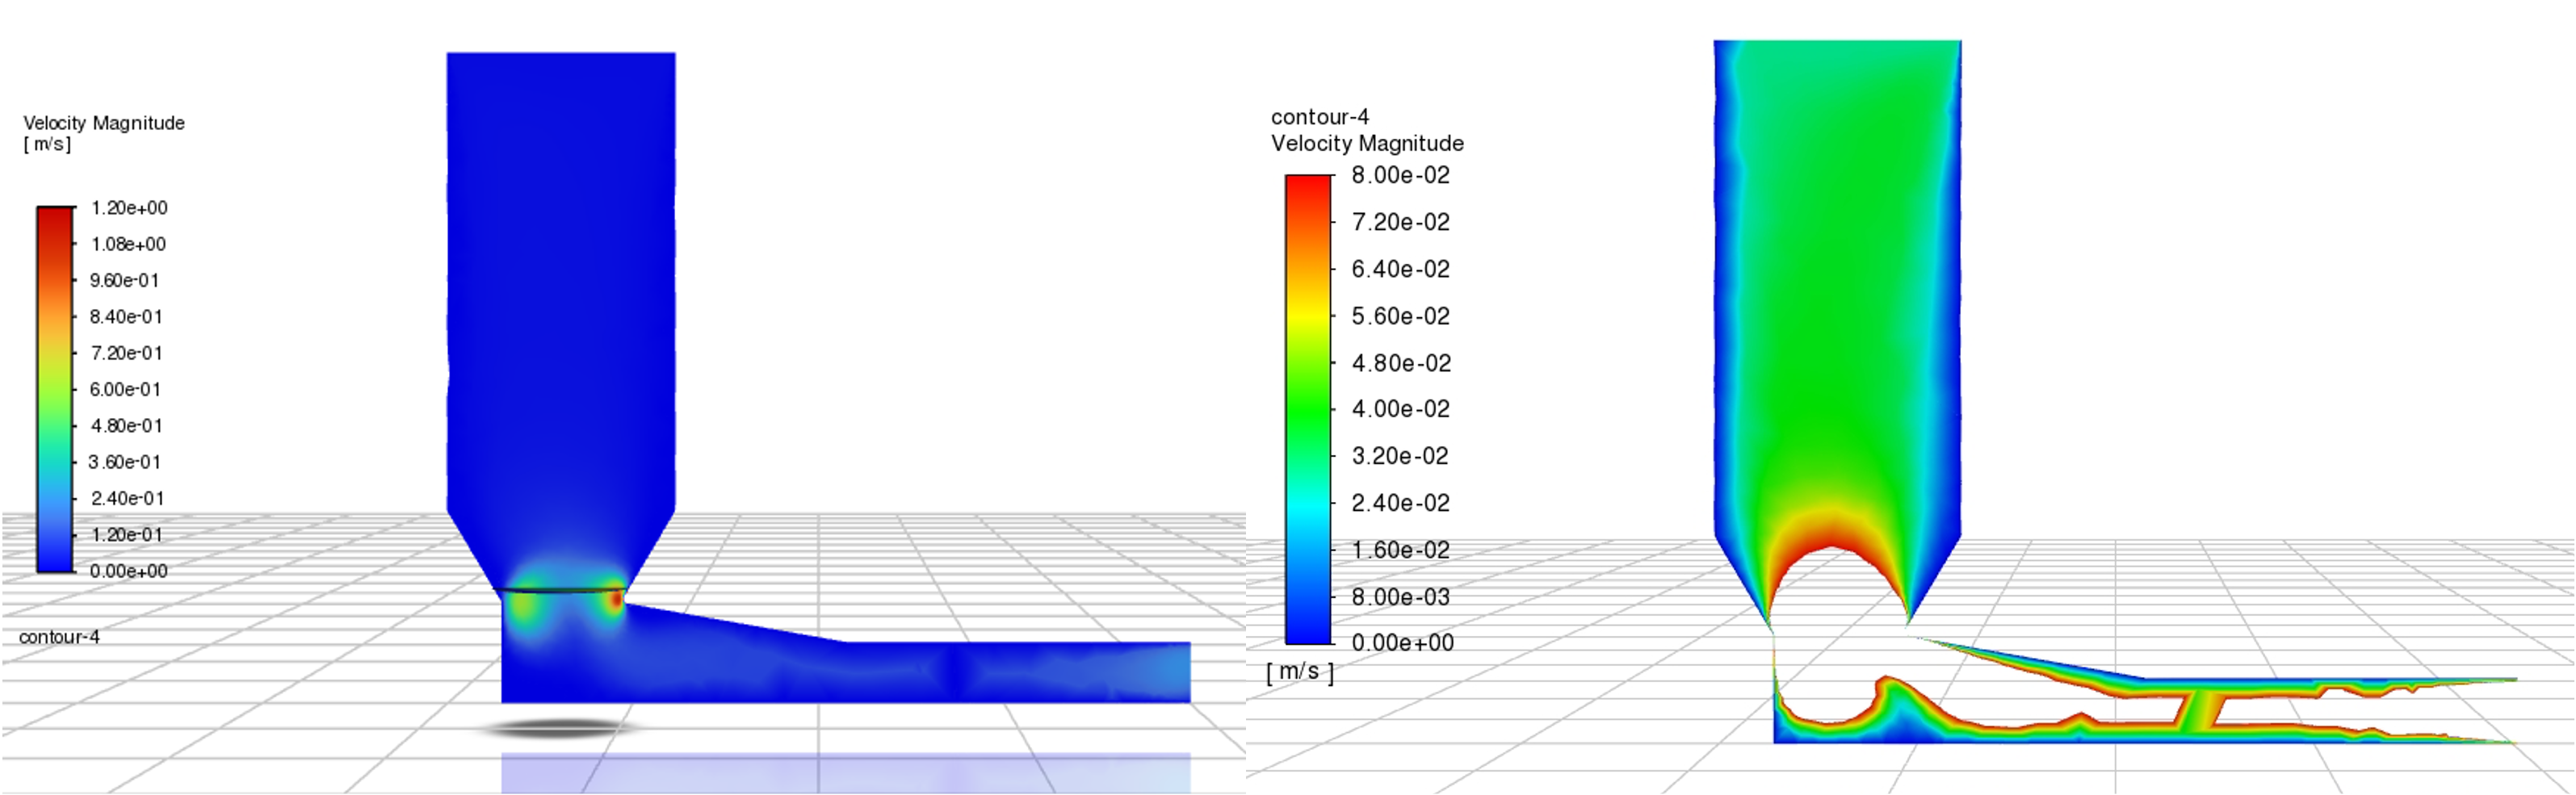
\includegraphics[width=0.85\textwidth]{figures/3.1.png}
  \caption{基准工况纵截面（XY平面）速度云图与细节图}
  \label{fig:3.1}
\end{figure}

未屈服插塞区的半径$r_{plug}$可通过壁面剪切应力$\tau_{wall}$估算。对于管道流动中的黏塑性流体，径向力平衡要求切应力沿径向线性分布，当管道中心切应力降低至等于屈服应力$\tau_0$时，即为插塞区边界，由此得到插塞区半径比的近似关系：
\begin{equation}\label{eq:rplug}
  \frac{r_{plug}}{R} = \frac{\tau_0}{\tau_{wall}},
\end{equation}
其中$R$为管道半径，$\tau_{wall}$可从CFD计算结果的喷嘴出口壁面剪切应力中提取。

基准工况下$\tau_{wall} \approx 84.93$~Pa，$\tau_0 = 500$~Pa，由\cref{eq:rplug}可得$r_{plug}/R \approx 5.9 > 1$。这说明在此工况下，喷嘴出口直管段中截断条件已基本满足，整个截面接近完全屈服状态，这与速度云图中出口截面速度分布较为均匀的观察一致。

进入收缩段后，流道截面积沿流动方向（-Y方向）单调减小，由质量守恒方程（连续性方程）可知，流速随之加速。出口截面（$D_{out} = 26$~mm）处最大流速约为1.3134~m/s，约为入口流速（0.03~m/s）的44倍，与入口截面积与出口截面积之比（$D_{in}^2 / D_{out}^2$）基本吻合，验证了质量守恒的合理性。收缩段内的强烈剪切作用使浆体屈服区域显著扩大，有利于提高挤出均匀性。收缩段喷嘴出口处的速度分布图如\cref{fig:3.2}所示。

\begin{figure}[!htb]
  \centering
  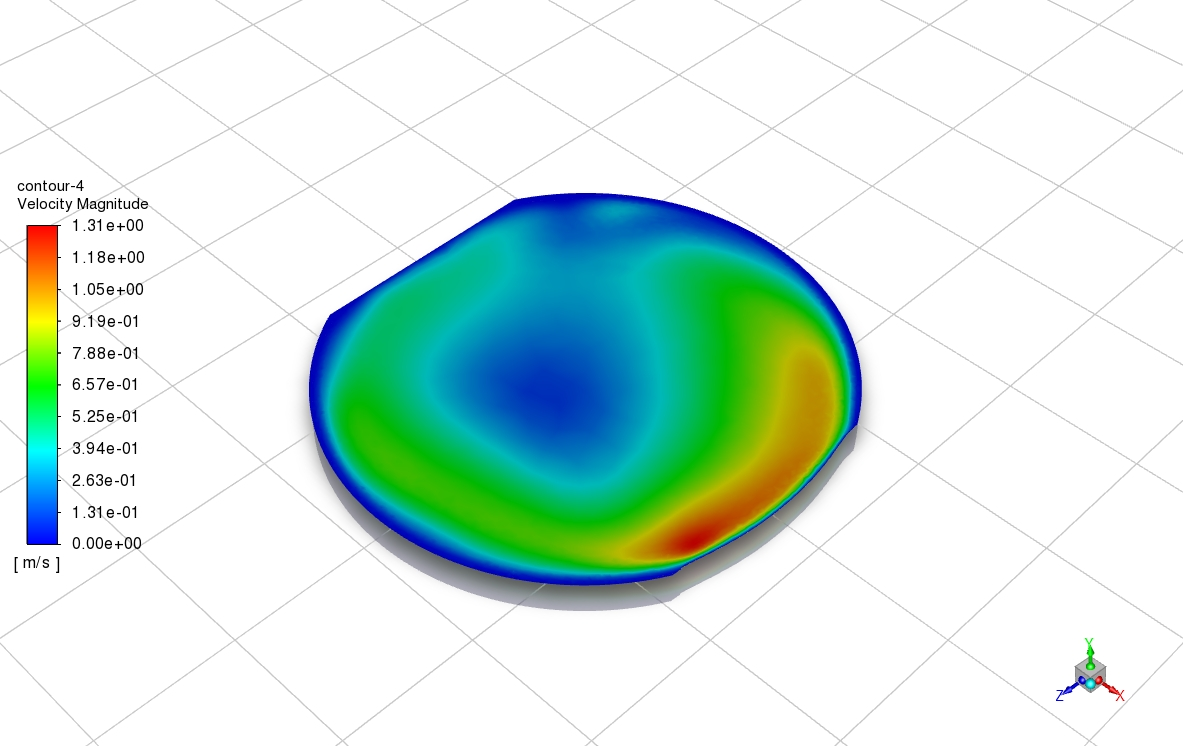
\includegraphics[width=0.7\textwidth]{figures/3.2.jpg}
  \caption{收缩段喷嘴出口处速度分布图}
  \label{fig:3.2}
\end{figure}

\subsection{整形板区域速度特征}

喷嘴的三维流线图如\cref{fig:3.3}所示。混凝土浆体离开喷嘴出口后，原本竖直向下（-Y方向）的方向在前挡板的阻挡作用下发生强制转折，转变为沿打印方向（+X方向）的横向流动。这一方向转折过程伴随着流场的剧烈重组：浆体在前挡板附近产生明显的滞止区，动压部分转化为静压，形成局部高压区。而这个局部高压区则正是基底面接触压力产生的核心驱动机制。

\begin{figure}[!htb]
  \centering
  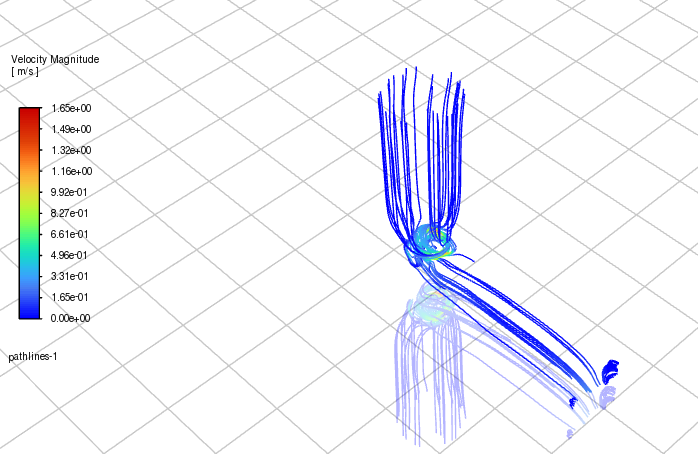
\includegraphics[width=0.75\textwidth]{figures/3.3.png}
  \caption{喷嘴三维流线图（Pathline）}
  \label{fig:3.3}
\end{figure}

在整形板受限区内，流体同时受到顶板（上方约束）、左右侧板（横向约束）和倾斜出料段（下方约束）的四面围合作用，形成封闭的楔形流动通道。受限空间内的几何约束使流体静压力得到积累，并通过倾斜出料段末端开口压向基底面，产生有效的层间接触压力。

\cref{fig:3.4}给出了整形板末端出料口的速度分布云图。由图可见，出料口截面的速度分布较为均匀，截面中心与边缘速度差较小（0.13~m/s），说明经过整形板的约束与整形作用，挤出物在离开整形板时具有较好的流动均匀性，有利于沉积层几何形态的稳定。

\begin{figure}[!htb]
  \centering
  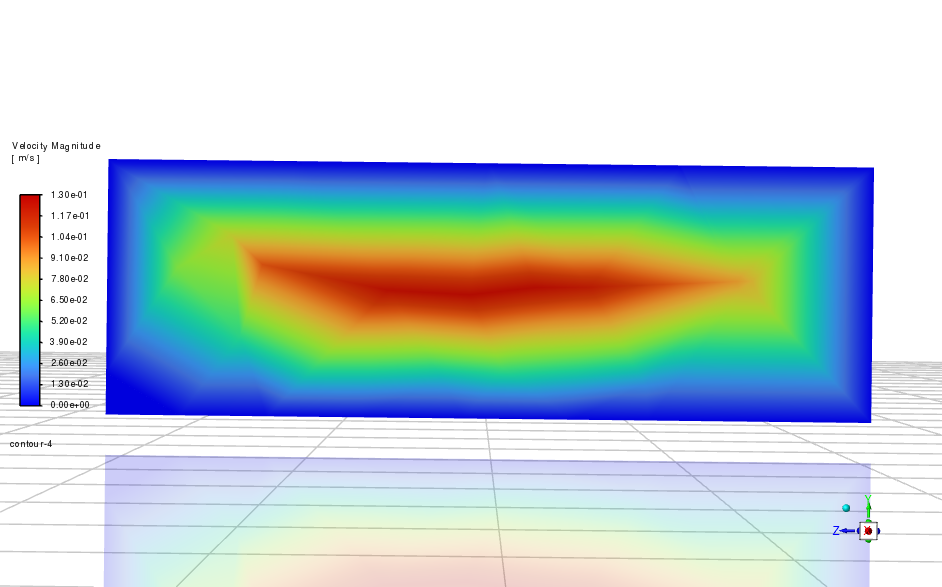
\includegraphics[width=0.7\textwidth]{figures/3.4.png}
  \caption{整形板末端出料口速度分布云图}
  \label{fig:3.4}
\end{figure}

\section{压力场分析}

\subsection{整体压力分布}

\cref{fig:3.5}与\cref{fig:3.6}分别展示了基准工况下喷嘴纵截面的压力云图与沿流动路径各监测截面的面积加权平均（Area-Weighted Average, AWA）静压力分布折线图。

\begin{figure}[!htb]
  \centering
  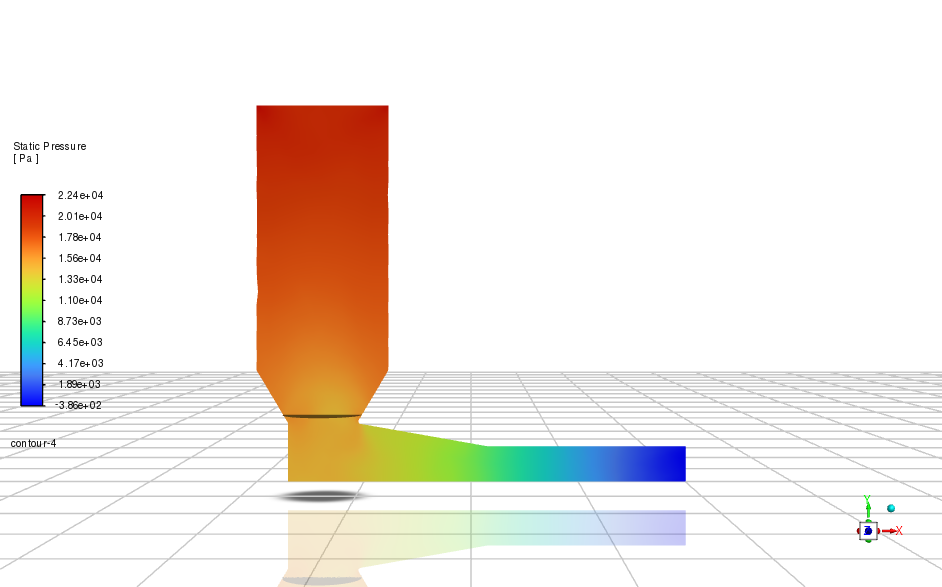
\includegraphics[width=0.7\textwidth]{figures/3.5.png}
  \caption{基准工况纵截面压力云图}
  \label{fig:3.5}
\end{figure}

\begin{figure}[!htb]
  \centering
  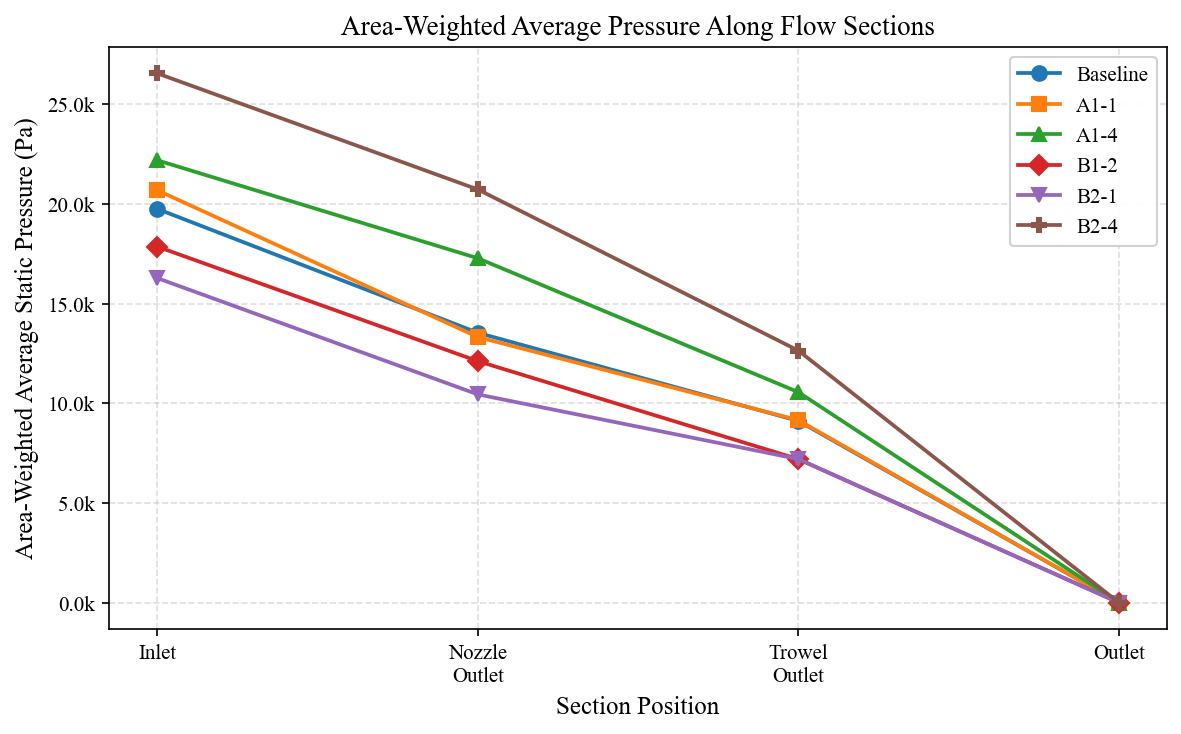
\includegraphics[width=0.8\textwidth]{figures/3.6.png}
  \caption{各截面面积加权平均压力折线图}
  \label{fig:3.6}
\end{figure}

由图可见，压力沿流动方向（从入口到出口）呈单调递减分布，这一趋势符合黏性流体流动的基本规律，驱动流体流动的压力梯度由入口泵送系统提供，并沿程克服流动阻力耗散。各截面面积加权平均压力的具体数值见\cref{tab:3.2}。

\begin{table}[!htb]
  \centering
  \caption{基准工况各截面压力汇总表}\label{tab:3.2}
  \renewcommand{\arraystretch}{1.3}
  \begin{tabular}{lccc}
    \toprule
    \textbf{截面} & \textbf{面积加权平均压力(Pa)} & \textbf{Max(Pa)} & \textbf{Min(Pa)} \\
    \midrule
    入口截面         & 19750     & 21874 & 18364 \\
    喷嘴出口截面     & 13536     & 15028 & 11830 \\
    整形板出口截面   & 9114      & 10442 & 8517 \\
    延伸段出口截面   & $\sim 0$  & 0     & -23.7 \\
    基底面           & 8310      & 13983 & -775 \\
    \bottomrule
  \end{tabular}
\end{table}

各流动区段的压降详细分析如下：

（1）收缩段压降：从喷嘴入口面（19750~Pa）至喷嘴出口面（13536~Pa），压降为5614~Pa，占总压降的约27\%。该区域压降主要由流道截面积的急剧减小引起，伴随流速大幅提升，黏性耗散显著增大。

（2）整形板受限区压降：从喷嘴出口面（13536~Pa）至整形板出口面（9114~Pa），压降为5076~Pa，约占25\%。该区段内流体受整形板四面约束，流动方向发生90°转折，局部流动阻力较大，压降集中。

（3）延伸段压降：从整形板出口面（9114~Pa）至延伸段终点（$\approx 0$~Pa），压降为9114~Pa，占46\%，是三段中最大的。模型试验中设计的75~mm延伸段并非约束区域，压力在此逐渐释放至环境压力。该区段的设置在物理上是必要的，因为如果缺少延伸段而直接在整形板末端施加出口边界条件，将导致整形板出口面处压力场失真，影响整形板约束区的计算精度，这也是本课题在几何建模时专门设置75~mm延伸段的原因。

在整形板受限区内，前挡板处动压向静压的转化是产生基底接触压力的核心机制。具体而言，浆体以较高速度（约1~m/s量级）冲击前挡板，动能转化为压力势能，在前挡板附近形成局部高压区，该高压通过流体内部压力传递作用于下方的基底面，产生层间接触压力。

\subsection{基底面压力沿打印方向分布}

基底面（Substrate，俯视XZ平面）的压力云图如\cref{fig:3.7}所示，基底面压力沿打印方向（X轴）的分布曲线如\cref{fig:3.8}所示。这两张图共同揭示了整形板约束作用下基底接触压力的空间分布特征，是本文参数化研究中各工况对比分析的基准参照。

\begin{figure}[!htb]
  \centering
  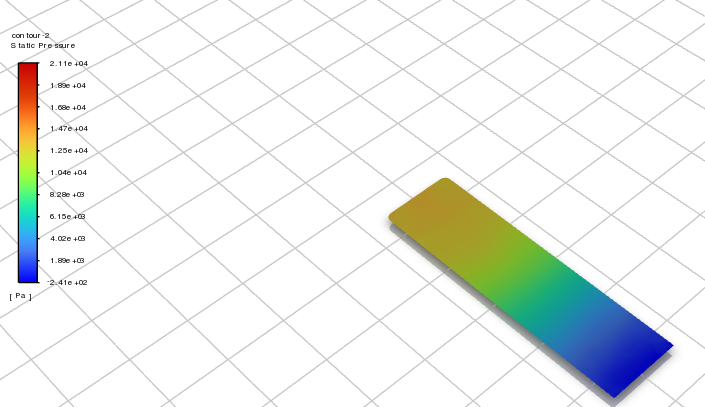
\includegraphics[width=0.75\textwidth]{figures/3.7.png}
  \caption{基底面（Substrate）压力云图（俯视，XZ平面）}
  \label{fig:3.7}
\end{figure}

\begin{figure}[!htb]
  \centering
  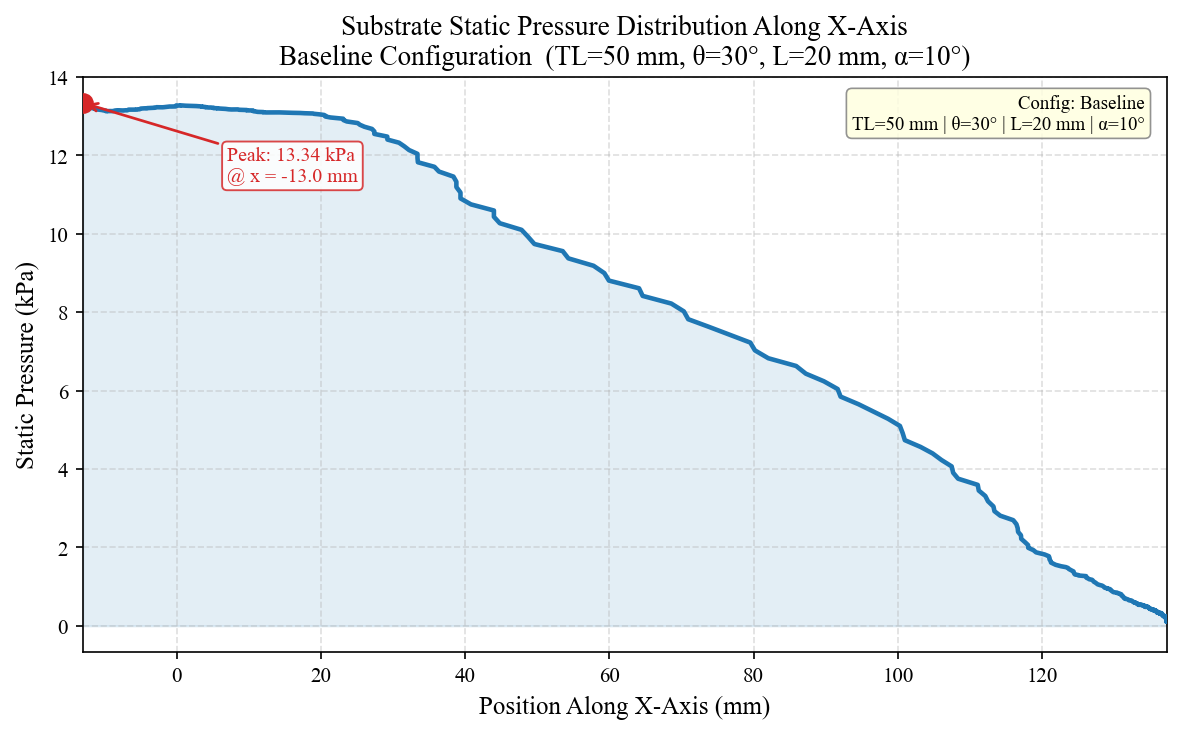
\includegraphics[width=0.8\textwidth]{figures/3.8.png}
  \caption{基底面压力沿X轴分布曲线（基准工况）}
  \label{fig:3.8}
\end{figure}

由\cref{fig:3.7}所示，基底面压力分布具有明显的空间非均匀性：高压区集中于整形板约束区域的中心偏前部，对应喷嘴出口正下方区域（$X \approx 0$附近），面积加权平均压力达到8310~Pa，最大压力峰值为13983~Pa。

\cref{fig:3.8}的XY曲线提供了更清晰的沿程分布信息。压力从整形板入口端（$X \approx 0$）的峰值13983~Pa开始，沿打印方向（+X方向）随着流体远离高压约束区而逐渐衰减，在延伸段末端附近，压力降至接近零甚至出现轻微负值（$-775$~Pa）。基底面压力在前26~mm出现了一个平台期，而这部分区域也正是喷嘴出料口面的宽度；随后，沿程压力得到了逐步释放。

基底面压力负压区的出现具有明确的物理成因：浆体流经整形板末端时，受约束突然释放，流体在出料口后缘发生局部流动分离，导致局部压力低于环境压力。负压区的量值较小（$<1$~kPa），对整体接触压力的评估影响有限，但其存在说明整形板末端的几何形状（倾斜角$\alpha$）对该区域的压力分布有显著影响，将在\cref{chap:parametric}第\ref{sec:alpha-influence}节的参数化分析中进一步讨论。

\section{剪切应力与黏度分布}

\subsection{剪切速率分布与插塞流区域}

\cref{fig:3.9}给出了基准工况下喷嘴纵截面的剪切速率分布云图。

\begin{figure}[!htb]
  \centering
  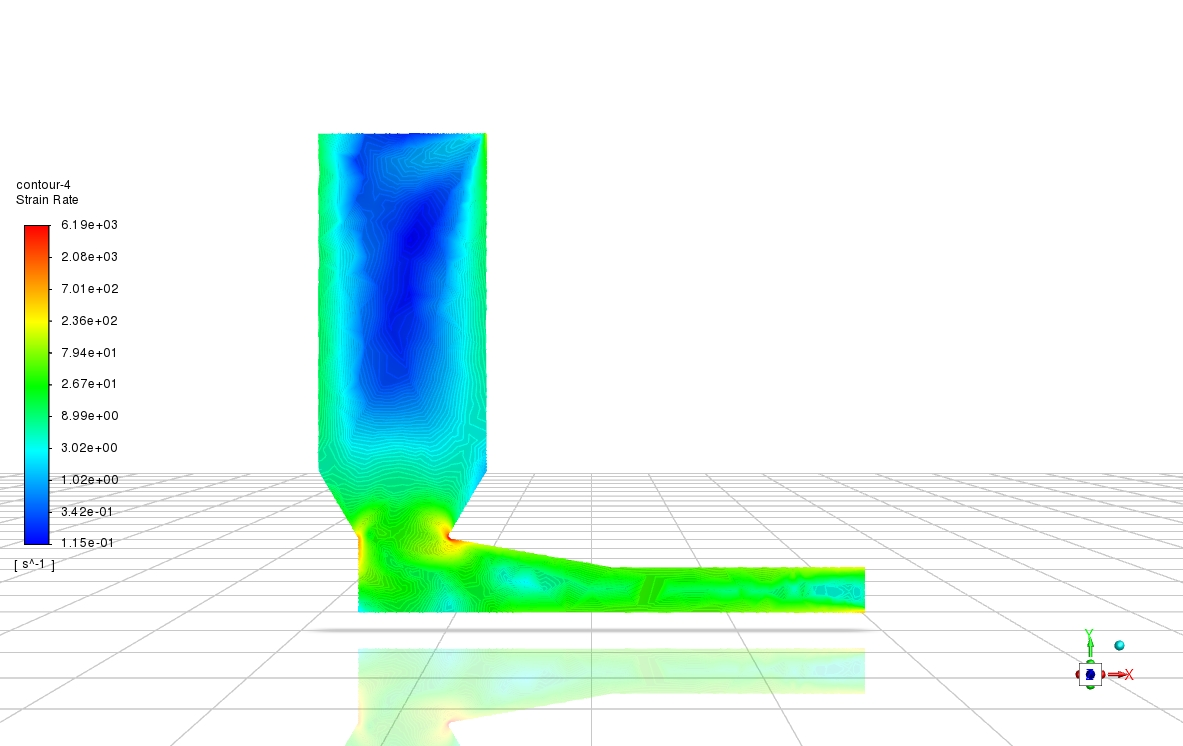
\includegraphics[width=0.7\textwidth]{figures/3.9.jpg}
  \caption{剪切速率分布云图（纵截面）}
  \label{fig:3.9}
\end{figure}

在CFD计算中，局部剪切速率$\dot{\gamma}$由应变速率张量$\mathbf{D}$的二阶不变量定义：
\begin{equation}\label{eq:shear-rate}
  \dot{\gamma} = \sqrt{2 \mathbf{D} : \mathbf{D}},
\end{equation}
\begin{equation}\label{eq:strain-rate}
  \mathbf{D} = \frac{1}{2} (\nabla \mathbf{u} + \nabla \mathbf{u}^T).
\end{equation}
由\cref{fig:3.9}可见，剪切速率的空间分布高度不均匀，呈现出显著的分区特征：

高剪切速率区（$\dot{\gamma} \gg \dot{\gamma}_c$）主要集中于两个位置：（1）喷嘴收缩段的近壁区域：喷嘴收缩段壁面急剧收缩，近壁区域的速度梯度最大，最大剪切速率达到6190~s⁻¹；（2）整形板受限区与前挡板附近：流体在此处经历强制方向转折，局部速度梯度同样较大。

低剪切速率区（$\dot{\gamma} < \dot{\gamma}_c$，未屈服plug zone）则占据入口直管段的中心区域，以及整形板受限区中流速较为均匀的区段。

这种剪切速率的分区分布对打印质量具有双重意义：一方面，高剪切区内浆体已充分屈服，流动阻力较低，有利于挤出顺畅；另一方面，过高的剪切速率会导致浆体结构破坏，可能降低早龄期强度，不利于沉积后的形状保持。因此，合理控制喷嘴内的剪切速率分布是喷嘴设计优化的重要目标之一。

\subsection{黏度场与屈服区}

黏度场分布云图如\cref{fig:3.10}所示。

\begin{figure}[!htb]
  \centering
  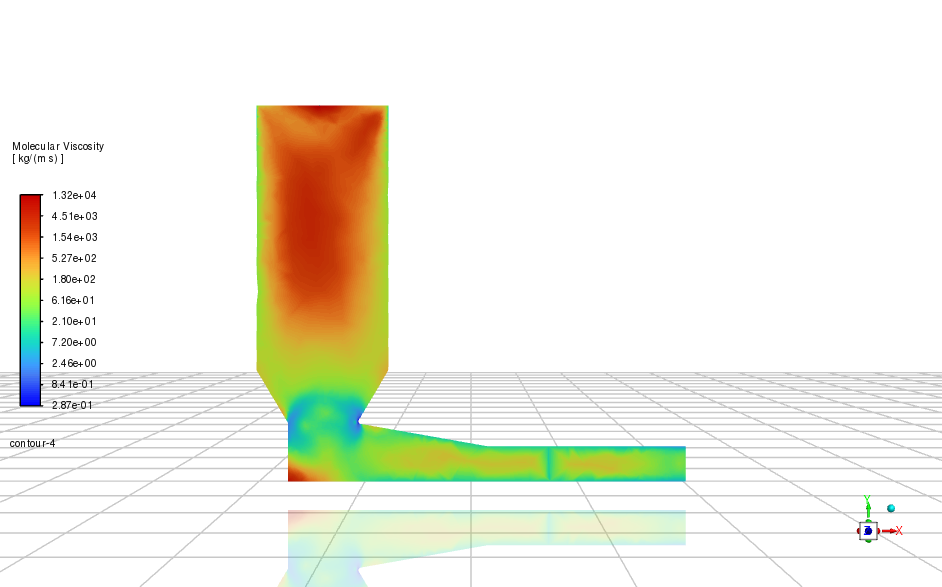
\includegraphics[width=0.7\textwidth]{figures/3.10.png}
  \caption{黏度分布云图（纵截面）}
  \label{fig:3.10}
\end{figure}

由H-B本构模型可知，表观黏度$\eta$与剪切速率$\dot{\gamma}$存在一一对应关系：剪切速率越高，表观黏度越低（剪切变稀）；在未屈服区（$\dot{\gamma} \leq \dot{\gamma}_c$），黏度取截断上限值为$\eta_{max} = 50000$~Pa·s，近似模拟固体行为。

由图可见，黏度场与剪切速率场呈镜像对应关系：喷嘴中心未屈服区黏度接近$\eta_{max}$（图中深色区域），而收缩段近壁高剪切区黏度降低3-4个数量级，最低可至$\eta_{min} = 1$~Pa·s附近（图中浅色区域）。这一量级的黏度差异（约$10^4$倍）是非牛顿流体CFD模型的典型特征，也验证了H-B模型的Papanastasiou正则化处理在本工况下使用的合理性。

\cref{fig:3.11}进一步通过布尔提取的方式，直观展示了屈服区（$\dot{\gamma} > \dot{\gamma}_c$，图中红色）与未屈服区（$\dot{\gamma} \leq \dot{\gamma}_c$，图中蓝色）的空间边界。从层间粘结的角度来看，已屈服的浆体具有一定的流动性，沉积时有利于与前一层浆体发生界面融合，提升层间粘结强度；而大量未屈服材料的存在则有利于沉积后的形状保持，防止层体在自重作用下坍塌。因此，屈服区与未屈服区的合理分布对于3D打印质量具有重要意义，喷嘴几何参数（尤其是收缩角$\theta$）对这一分布的影响将在\cref{chap:parametric}中进一步量化分析。

\begin{figure}[!htb]
  \centering
  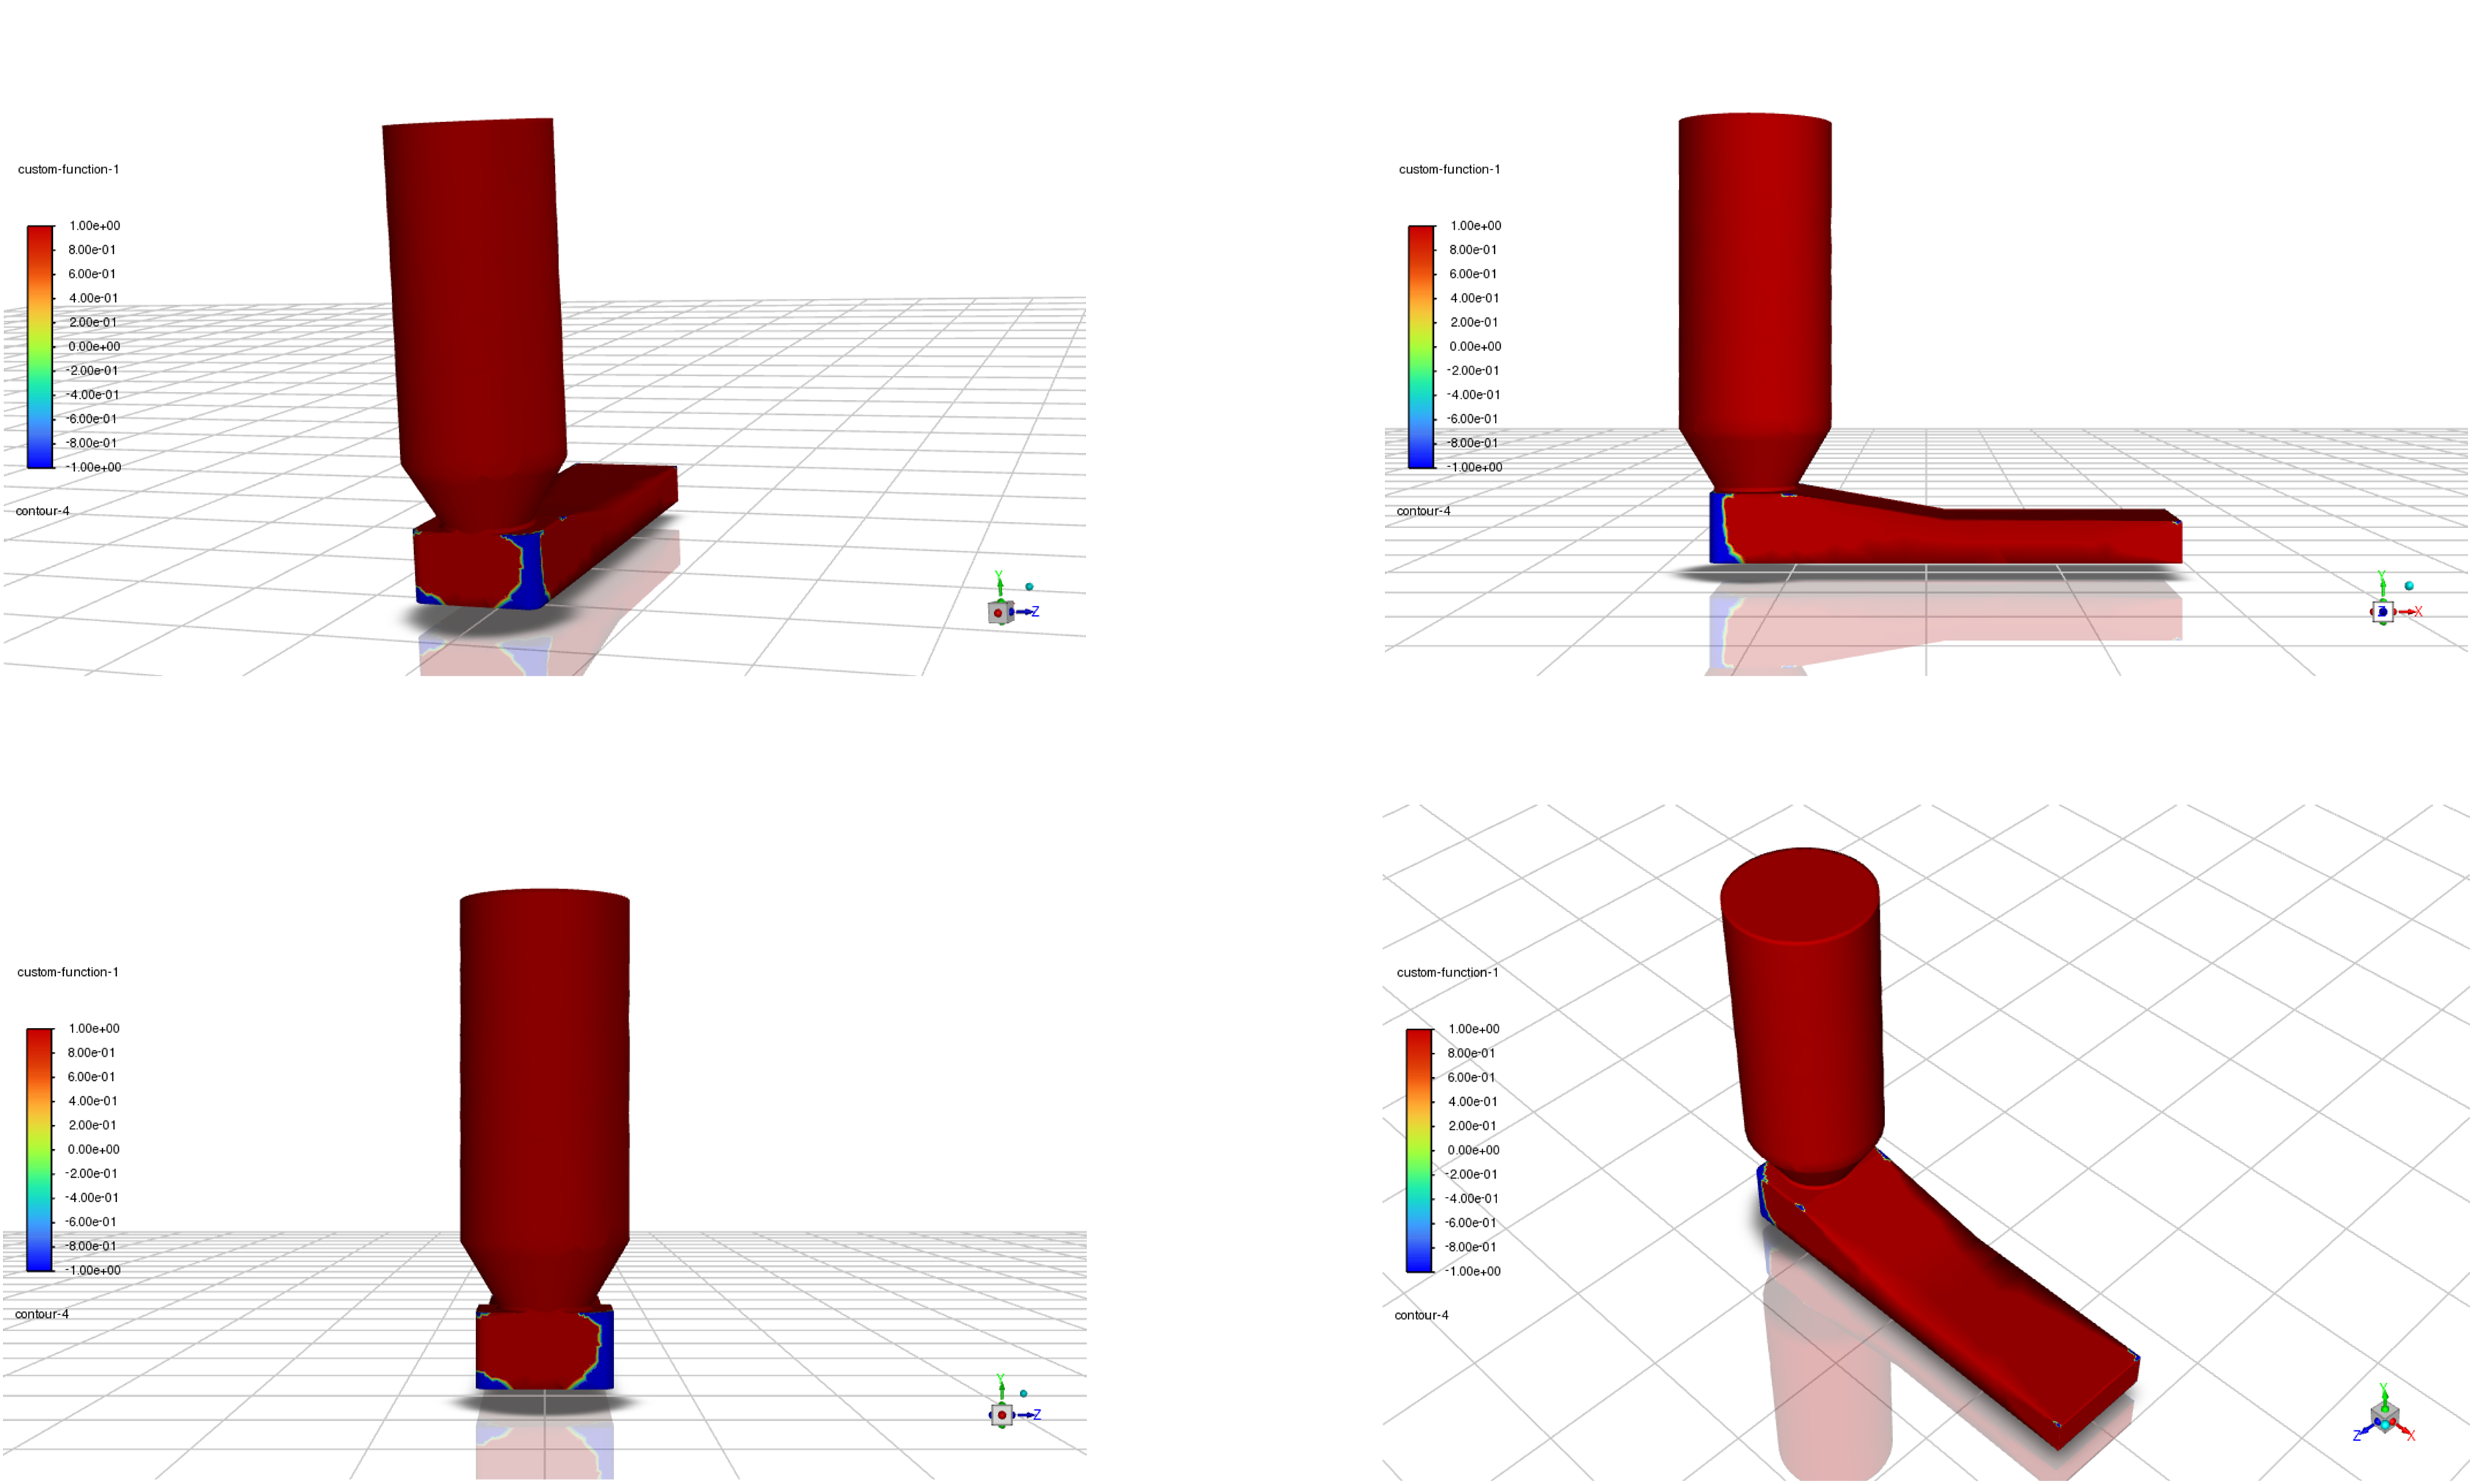
\includegraphics[width=0.7\textwidth]{figures/3.11.png}
  \caption{屈服区/未屈服区分布示意图（布尔提取）}
  \label{fig:3.11}
\end{figure}

\subsection{壁面剪切应力}

壁面的壁面剪切应力（Wall Shear Stress, WSS）分布云图如\cref{fig:3.12}所示。壁面剪切应力反映了浆体在壁面附近的黏性阻力强度，是喷嘴磨损寿命预测和材料剪切损伤评估的重要参数。

\begin{figure}[!htb]
  \centering
  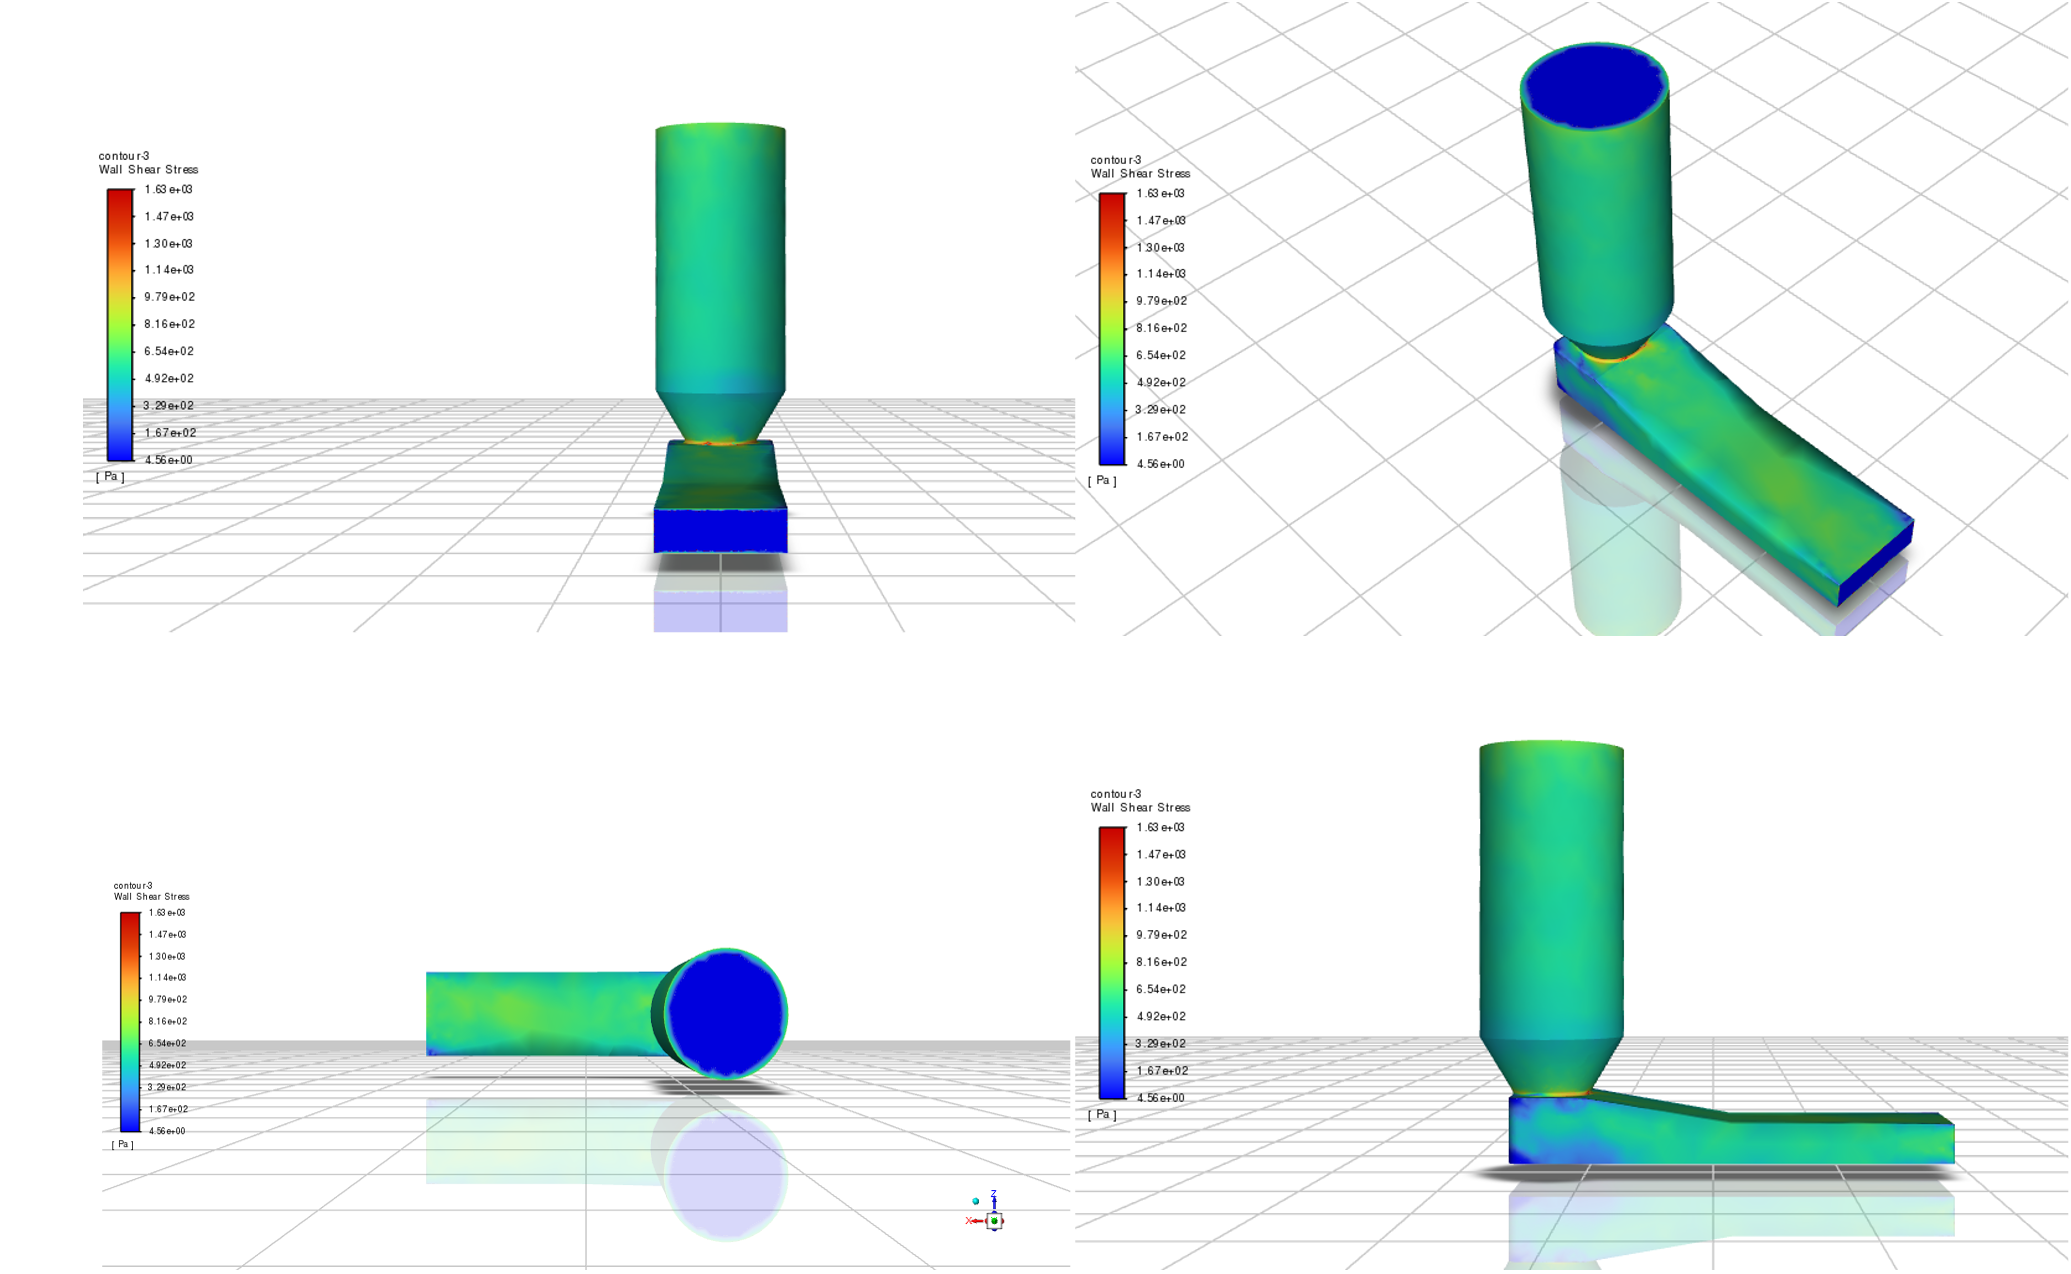
\includegraphics[width=0.75\textwidth]{figures/3.12.png}
  \caption{壁面剪切应力分布云图}
  \label{fig:3.12}
\end{figure}

由\cref{fig:3.12}及\cref{tab:3.2}中的定量数据可知，各壁面的壁面剪切应力分布存在显著差异。喷嘴出口截面的面积加权平均壁面剪切应力为84.9~Pa，反映了喷嘴内壁在出口段承受的平均剪切载荷；整形板末端出料口的面积加权平均壁面剪切应力则为172.7~Pa，高于喷嘴出口，这是因为整形板末端流道截面积较小（受倾斜角$\alpha$约束），流速梯度更大，壁面剪切载荷相应增大。从喷嘴设计的工程角度来看，壁面剪切应力越大，喷嘴固件的磨损就越快、材料就会越容易受到剪切破坏。因此，在追求高接触压力的同时，还需兼顾对壁面剪切应力的控制。

基底面的壁面剪切应力则反映了浆体对已打印层基底面的切向作用力。该值过大可能导致基底表面材料被撕裂或已打印层结构被破坏，是评估打印工艺对已沉积层影响的重要指标。
